Avant de définir une stratégie de documentation pour le projet Buckless, nous allons
nous intéresser à la manière dont les différents outils présentés précédemment ont été
intégrés par de gros projets open source.\\
Ces projets ont été choisis pour leur similitude avec le projet Buckless, que ce soit
par les technologies utilisées, le type de logiciel produit, l'architecture logicielle
semblable, etc.

\subsection{Nylas N1}
    \subsubsection{Présentation}
        Nylas est une organisation réalisant le projet N1, un client mail se basant sur des technologies web.
        En effet, le projet utilise un chromium\footnote{Navigateur web} embarqué  pour distribuer une application
        web en tant qu'application native. Cela permet d'avoir une interface facilement stylisable et extensible,
        en plus d'être multiplateforme et portable.\\
        Cette interface utilise une API REST, ouverte, dont la documentation est générée à partir du code.
        Malheureusement, le code source de cette API n'est pas disponible et il n'y a pas moyen de connaître la méthode de génération.
        On peut toutefois observer que la génération de la documentation est faite en interne via un script,
        et non automatiquement à l'aide d'intégration continue.

    \subsubsection{Stratégie de documentation}
        \paragraph{}
            Une documentation est aussi disponible pour l'application en elle-même.
            Vu que le projet est basé sur le paradigme de Programation Orienté Objet, les classes sont assez facile à identifier avec "l'API Reference".
            De plus, N1 utilise les Web Components — qui apportent la modularité aux sites webs en découpant chaque partie en composants autonomes,
            et ils sont eux aussi facilement identifiables.

        \begin{figure}[ht]
            \centering
            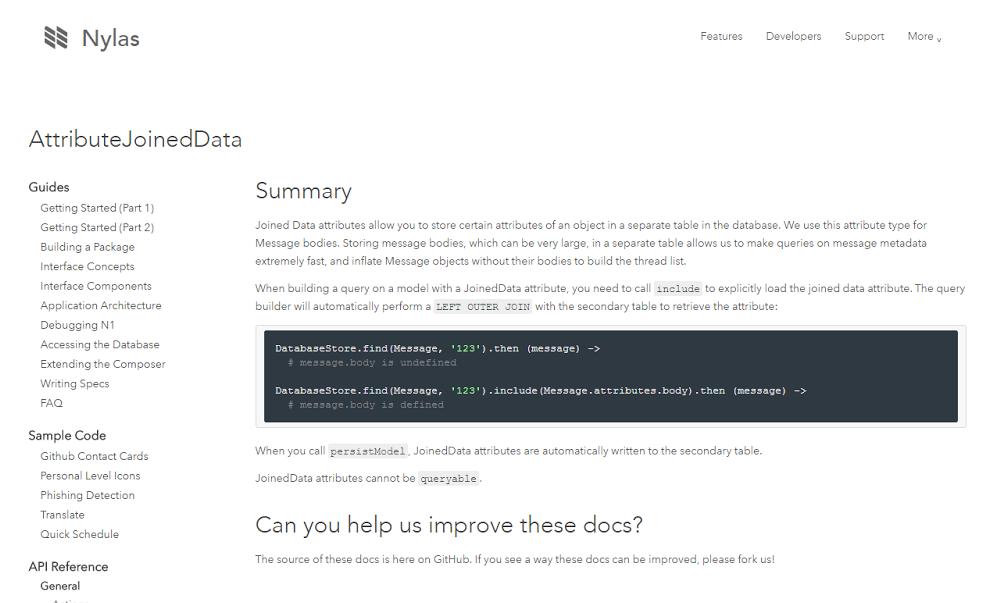
\includegraphics[scale=0.35]{./assets/nylasdoc2.png}
            \caption{Acceuil de la documenation}
        \end{figure}

        \paragraph{}
            L'intérêt majeur de cette documentation est qu'elle est générée via le code source de l'application.
            En utilisant les commentaires, leur script de génération de documentation va créer une arbre syntaxique (AST\footnote{Abstract Syntax Tree}),
            aussi utilisé dans la compilation de programmes.

        \begin{figure}[h]
            \centering
            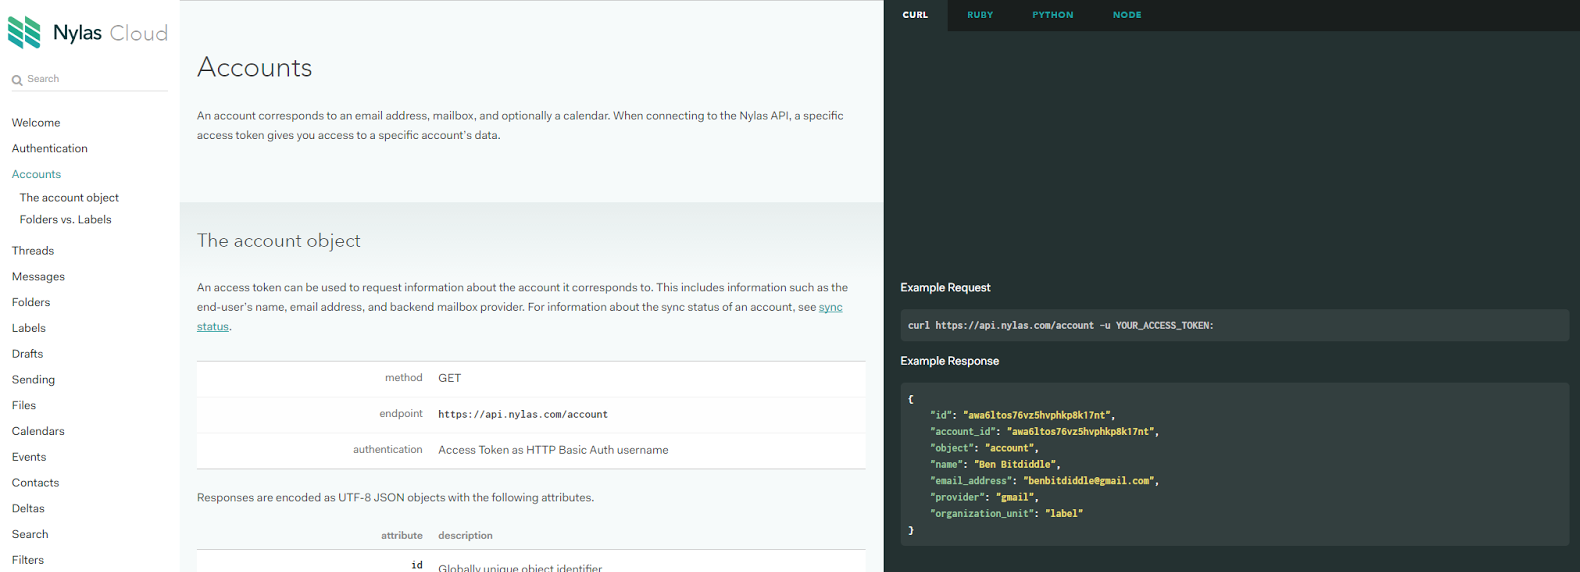
\includegraphics[width=\textwidth]{./assets/nylasdoc.png}
            \caption{La référence de l'API}
        \end{figure}

        \begin{listing}[ht]
            \begin{minted}[
                bgcolor=black,
                fontsize=\footnotesize
            ]{ruby}
# Public: A mutable text container with undo/redo support
class TextBuffer
  @prop2: "bar"

  # Public: Takes an argument and does some stuff.
  #
  # a - A {String}
  # Returns {Boolean}.
  @method2: (a) ->
            \end{minted}
            \caption{Exemple de commentaire TomDoc}
        \end{listing}

        \paragraph{}
            Au niveau des commentaires, un dérivé de jsDoc (TomDoc\cite{tomdoc}) est utilisé, plus adapté
            pour des grosses parties de documentation (là où jsDoc est plus adapté pour l'auto complétion et la documentation rapide).
            La génération de l'AST est faite à l'aide d'une librairie spécialisée\cite{donna}.
        \begin{listing}[ht]
            \begin{minted}[
                bgcolor=black,
                fontsize=\footnotesize
            ]{json}
"files": {
"spec/metadata_templates/classes/class_with_prototype_properties.coffee": {
  "objects": [
        "type": "class",
        "name": "TextBuffer",
        "bindingType": null,
        "classProperties": [],
        "prototypeProperties": [11, 11],
        "doc": " Public: A mutable text container with undo/redo support\n\n "
[...]
            \end{minted} \caption{Une partie de l'AST produit sous forme de JSON}
        \end{listing}

        \paragraph{}
            L'AST généré est ensuite transformé en code quasiment exportable en HTML, en utilisant une deuxième librairie\cite{tello}.
            Enfin, Nylas possède un script qui va automatiquement réaliser l'AST puis le contenu et générer le code HTML de la documentation.
            Le code est ensuité publié sur une branche spécifique à la documentation de leur projet.
            Cette branche est automatiquement mise en ligne par GitHub\cite{ghpages} ce qui permet uniquement en
            modifiant le code, de mettre à jour la documentation en ligne directement.

\subsection{Ghost}
    \subsubsection{Présentation}
        L'idée de Ghost est née lorsque Jon O'Nolan, fondateur de Wordpress, se rendit compte que
        Wordpress était devenu beaucoup trop complexe pour une simple plateforme de blogging. C'est
        à partir de ce constat qu'il décida de créer une plateforme de blogging dédiée uniquement au
        contenu. Débutant de projet de zéro, Ghost a été construit sur du javascript côté client et
        serveur.\\
        Ajourd'hui, Ghost est une plateforme massivement utilisée. C'est d'ailleurs un projet open-source,
        qui base son modèle économique sur du Software As A Service (SAAS). C'est donc autant pour les
        similitudes technologiques que celles du business model que Ghost a été retenu en tant qu'exemple.

    \subsubsection{Stratégie de documentation}
        \paragraph{}
            Contrairement à Nylas N1, Ghost a pris le parti de ne pas intégrer la documentation à sons processus
            de développement. La documentation est quelque chose de complètement indépendant du code,
            et possède son propre versionning. Ghost propose deux grands types de documentation : une documentation
            orientée utilisateur, et une orientée développeur. C'est sur cette dernière que va se concentrer
            notre analyse.

        \begin{figure}[h]
            \centering
            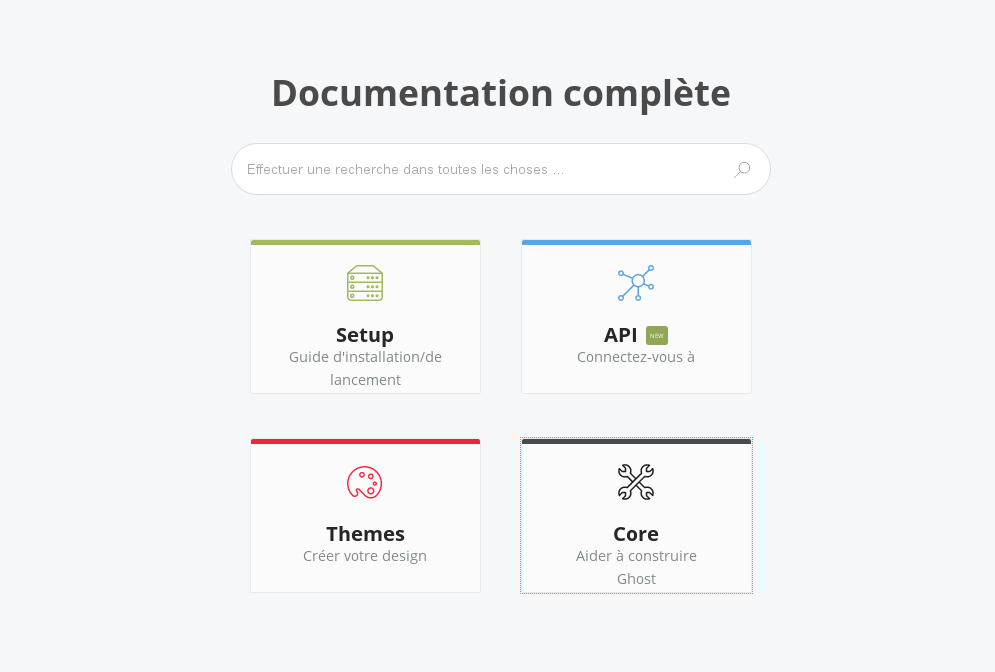
\includegraphics[scale=0.35]{./assets/ghost1.png}
            \caption{Acceuil de la documenation}
        \end{figure}

        \newpage
        \begin{figure}[h]
            \centering
            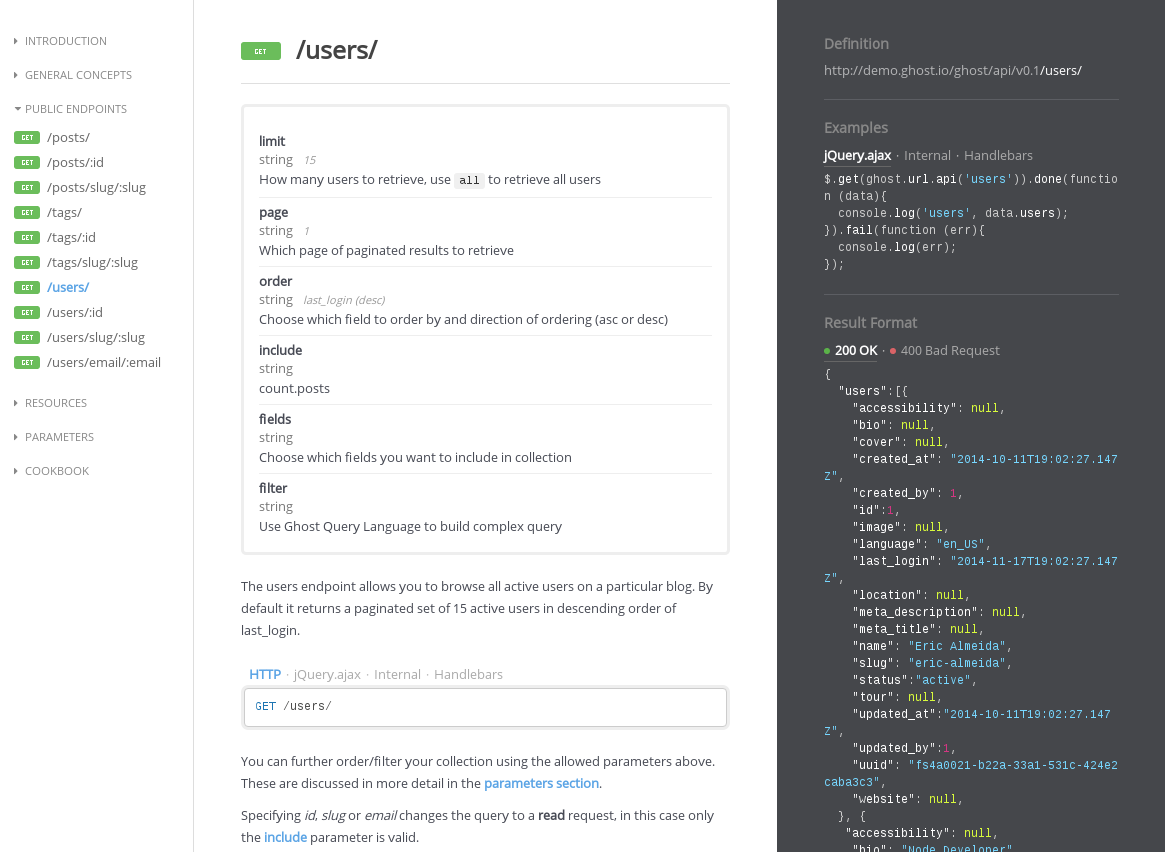
\includegraphics[height=12cm]{./assets/ghost2.png}
            \caption{API Reference}
        \end{figure}
        \paragraph{}
            Parmi la documentation développeur, deux grands axes sont développés.
            Le premier, est une documentation de l'API RESTful de Ghost. Un formalisme de description
            d'API tel que Swagger (probablement API Blueprint) est utilisé pour générer une documentation
            dynamique. Il n'est malheureusement pas possible d'en avoir la certitude, puisque la solution
            \footnote{readme.io} utilisée est payante.



        \newpage
        \paragraph{}
            Le deuxième est une documentation de la structure interne du serveur. Celle-ci aborde moins
            le côté "fonctionnel" du serveur, à savoir les différentes routes et ce qu'elles retournent, mais
            plus une approche structurelle qui permet de former les potentiels contributeurs. Elle
            décrit notemment le style de code à utiliser lors d'une contribution, l'architecture globale
            de l'application et ses composants, mais aussi des indications quant au déploiement de Ghost.
            Cette documentation se présente sous la forme d'un Wiki, hébergé directement sur le
            dépôt du projet sur GitHub. Différents types de documents sont proposés : du texte, des
            diagrammes et des schémas ASCII. On peut remarquer qu'aucun formalisme n'est utilisé
            pour les différents diagrammes.

        \begin{figure}[h]
            \centering
            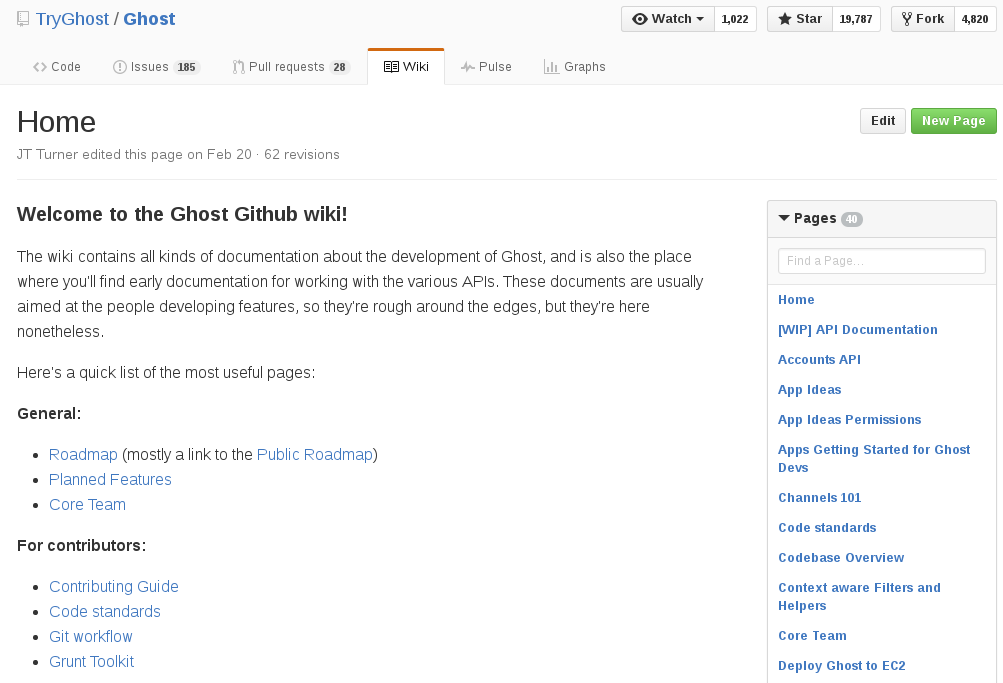
\includegraphics[height=12cm]{./assets/ghost3.png}
            \caption{Acceuil du wiki}
        \end{figure}

        Il est intéressant de constater les différences de stratégie de documentation des deux projets.
        D'un côté, Nylas N1 pousse la principe de la fusion des processus au maximum, en intégrant des
        paragraphes entiers de documentation au sein des commentaires de la source pour générer sa documentation.
        De l'autre, Ghost fait preuve d'une politique plus traditionnelle, en gardant complètement séparé
        l'action de développer et celle de documenter. Il est possible de voir ici des raisons économiques,
        puisque Ghost est un projet actuellement beaucoup plus gros. Ainsi, les ressources humaines sont
        également plus importantes et permettent d'avoir un pouvoir de développement et la capacité de
        pouvoir documenter en même temps sans avoir à se poser de question. Mais cela peut aussi être
        le résultat d'un choix, où l'automatisation de la documentation demande une grande part de
        configuration et l'utilisation d'une multitude d'outils, ce qui compléxifie le développement.\\
        C'est sur base de ces observations que nous allons maintenant essayer de définir une stratégie
        de documentation pour le projet Buckless.
